
\chapter{Procesamiento de Clickstream}
\label{logs}


\section{Introducción}

En un sitio Web, el análisis de \emph{``clickstream''} es el proceso de
recolección, análisis y presentación de datos agregados sobre cada paso
que siguen los visitantes en una página web y en qué orden, es decir,
son el resultado de la sucesión de clicks del ratón por cada visitante.
Regularmente, dicho flujo o registro de información es almacenado en un
principio para la gestión de los registros y posteriormente son
analizados para producir estadísticas que resulten de utilidad \citep{lagus2000text}.

%\section{ El problema por resolver}\label{el-problema-por-resolver}

En el caso de la biblioteca de arte, los registros de cada click que realizan los usuario en la página de DSpace son almacenados en un archivo común o estándar llamado  \href{https://httpd.apache.org/docs/2.2/logs.html}{access.logs}; estos archivos después de ser estructurados, tienen las principales ventajas de poder conocer a los usuarios y entender sus necesidades de búsqueda, conocer el día a día de las operaciones y en una segunda etapa poder realizar recomendaciones a los usuarios\citep{banerjee2002characterizing}.

Para realizar dicho análisis es necesario obtener y estudiar los datos provenientes de los access log\citep{apache} principalmente porque son datos no estructurados. Una vez estructurados, se necesitan quitar los registros duplicados, sesionizar los datos y enriquecer los registros ya que debido a las características que aporta cada registro, suelen no ser suficientes para tener un análisis más detallado.

Cabe destacar que no sólo la resolución del problema llega hasta esta fase, sino hasta la creación de un dashboard o tablero de estadísticas que ayudan a visualizar las principales características de los datos; por ejemplo, los usuarios que tienen más visitas, su tiempo de permanencia, las páginas más visitadas, entre otras.


\section{Orquestación}\label{orquestacion}

La orquestación se realiza por medio de \href{http://luigi.readthedocs.org/en/stable/}{luigi}, pero para el análisis de \emph{clickstream},  las ventajas que se utilizan son las de \emph{modularidad}, \emph{robustez} e \emph{idempotencia}. Cabe resaltar que para esta fase del proyecto, debido a que no se tienen archivos access log provenientes de \emph{D-space}, los archivos logs fueron obtenidos de diversas fuentes \citep{veterina}; sin embargo, la estructura típica de los access log es la misma para este tipo de archivos.
A continuación se describe los pasos del \emph{pipeline} que son ejecutados por la función principal \emph{analisis-log-itam.py}; en cada uno de estos se explica su función, así como también el archivo \emph{input} y \emph{output} necesario.


\subsubsection{ Inputlog}\label{i-inputlog}

Es el primer paso del pipeline y es el encargado de importar el archivo
\emph{access.logs} de la ruta predeterminada hacia el orquestador
(\emph{luigi}).

Como antecedente, este proceso se ejecutaba por medio de \emph{batch} en
el lenguaje de programación \emph{pearl} por medio de la función
\emph{accesslog2csv.pl}; sin embargo, se decidió integrar este paso a la
orquestación de \emph{luigi} para que el proceso se ejecutado en una
sola orquestación.


\begin{itemize}
\item \textbf{Input}: access.log
\item \textbf{Output}: inputlog.pd (archivo data frame pandas)
\end{itemize}




\subsubsection{ Parsear}\label{ii-parsear}

Después de que \emph{luigi} recibe el access.log,este paso es el
encargado de nombrar las variables y la estructura del archivo
\emph{access.log}. La estructura y los nombres de las variables fueron
tomadas de los \emph{CustomLog}
\href{https://httpd.apache.org/docs/2.2/logs.html}{apache.org}.

Las variables que se tienen son las siguientes:

\begin{itemize}
\itemsep1pt\parskip0pt\parsep0pt
\item
  Host: La dirección IP del usuario que accede al servidor web. \emph{127.0.0.1}
\item
  Log\_Name: El identificador de usuario en la máquina cliente \emph{frank}
\item
  Date\_Time
\item
  Method: Petición enviada por el cliente, inidicando el tipo (normalmente \emph{GET} o \emph{POST}).
\item
  Response\_Code: Código de respuesta de la página \emph{200}
\item
  Bytes\_Sent Es el número de bytes entregados por el servidor en la página de respuesta a la petición.
\item
  URL Es la página en donde se encuentra el enlace que ha generado la petición al servidor
\item
  User\_Agent: Es una cadena que identifica al navegador desde el cual se ha realizado la petición. 
\end{itemize}


\begin{itemize}
\item \textbf{Input}: inputlog.pd
\item \textbf{Output}: parsear.pd
\end{itemize}


\subsubsection{ Usuario}\label{iii-usuario}

En este paso se necesita tener identificados a los usuarios en sentido en la forma en que visitaran la página de DSpace ya que es el servicio de consulta de la biblioteca de arte, puede llevarse a cabo por medio de una computadora por usuario o varios usuarios en una misma computadora. La mejor práctica para identificar a los usuarios en este tipo de páginas, se realiza por medio de tablas intermedias como tablas de acceso, tablas de usuarios y tablas bitácora\citep{andersen2000analyzing}.

En caso de no existir este tipo de tablas intermedias, se tiene que trabajar por medio de suposiciones de como el usuario accede a la página, comúnmente se supone que cada usuario proviene de una IP única, si este no es el caso, se puede hacer el supuesto por medio de IP + buscador que utiliza y así sucesivamente; inclusive se puede hacer de forma heurística tomando en cuenta el tiempo entre páginas.

Para poder realizar este paso, nos basamos en el supuesto que un usuario, solo visitará el sitio por medio de una computadora o IP fija.

\begin{itemize}
\item \textbf{Input}: parsear.pd
\item \textbf{Output}: usuario.pd
\end{itemize}


Este paso es posible que sea modificado ya definida la estructura de
consulta de \emph{D-space}. Dentro de la función
\emph{analisis-log-itam.py} se tiene comentado en dónde se realizaría
dicho cambio.

\subsubsection{ Sesionizar}\label{iv-sesionizar}

La función de este paso es ordenar los registros por fecha y usuario,
quitar duplicados y agregar 2 campos nuevos que son:

\begin{itemize}
\item
  time\_diff: calcula la diferencia en tiempo entre una consultas del
  usuario en la página \emph{web} siendo el primer registro puesto como
  \emph{0} ya que no se tiene contra quien comparar.
\item
  Rank: crea un ``ranking'' entre las consultas por usuario, siendo
  \emph{1} la primera consulta del usuario, \emph{2} la segunda y así
  sucesivamente.
\end{itemize}

Para ejemplificar este paso, se tiene la siguiente tabla

\begin{table}[H]
\centering
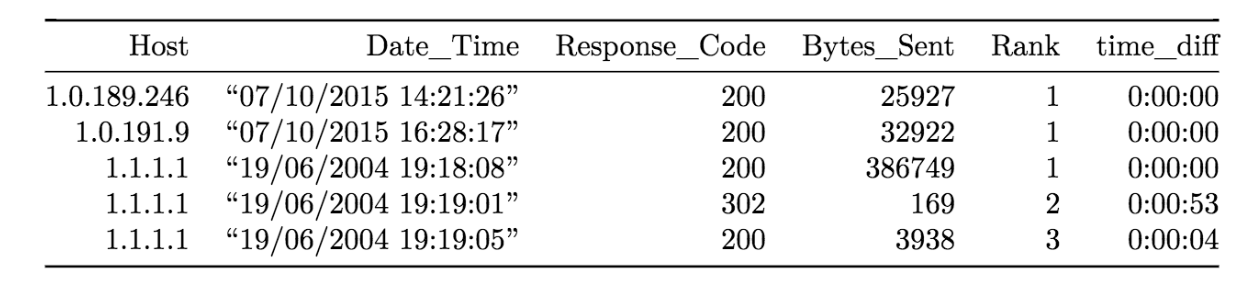
\includegraphics[width=0.8\textwidth]{Figures/tabla1.png}
\caption{Sesionizar}
\end{table}

Se observa que para el primer y segundo dato, sólo existe un registro de acceso en ese día, por lo que su $rank=1$ y su $time\_diff=0$; a partir del tercer datos, se observa que es un usuario con 3 registros, el rank es una secuencia de 1 a 3 en orden del tiempo y el campo de time diff siempre será 0 en el $rank=1$ y posteriormente realizará la diferencia entre registros.

\begin{itemize}
\item \textbf{Input}: usuario.pd
\item \textbf{Output}: sesionizar.pd
\end{itemize}



\subsubsection{Enriquecer}\label{v-enriquecer}

En este paso se crean nuevas variables o campos que podrían ser de
interés para el análisis. Los campos que se crean por consulta son los
siguientes:

\begin{itemize}
\itemsep1pt\parskip0pt\parsep0pt
\item
  year: año
\item
  month: mes
\item
  day: dia (número)
\item
  hour: hora
\item
  day of week: día de la semana
\item
  dif seg clicks: segundos de consulta
\end{itemize}

En este paso, pueden ser agregados más campos que sean de interés para
los administradores del sistema. Los campos descritos con anterioridad
son los más comunes ya que nos ayudan a determinar los días, horas, mes
y años de visitas más o menos frecuentes y/o el tiempo promedio de permanencia.

Un ejemplo de este paso sería el siguiente

\begin{table}[H]
\centering
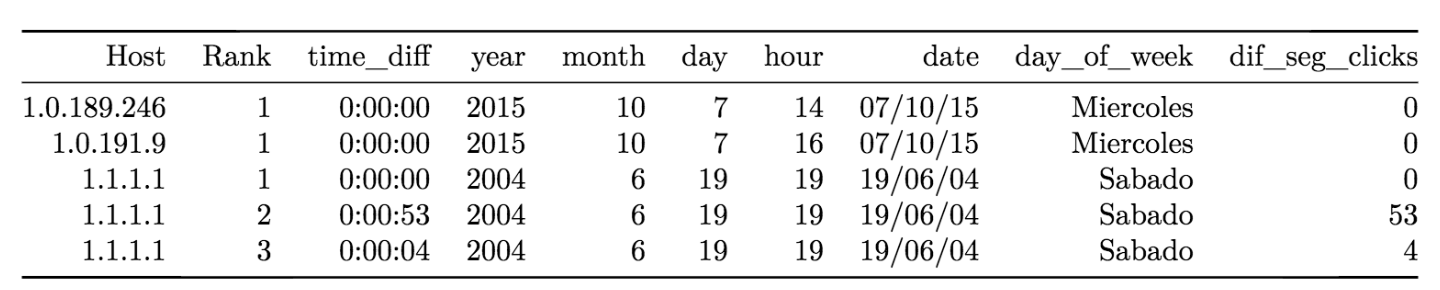
\includegraphics[width=1\textwidth]{Figures/tabla2.png}
\caption{Enriquecer}
\end{table}

El cual simplemente agrega campos que podrían ser de interés para el usuario. El output es de tipo \emph{csv} y es el insumo principal del dashboard.

\begin{itemize}
\item \textbf{Input}: sesionizar.pd 
\item \textbf{Output}: enriquecer.csv o enriquecer.pd
\end{itemize}


\subsubsection{ Reportes}\label{vi-reportes}

De manera automática son creados reportes en \emph{pdf} de los
\emph{códigos de respuesta} y \emph{usuarios} con las estadísticas del
porcentaje de visitas y el tiempo promedio de consulta.

\begin{itemize}
\item \textbf{Input}: enriquecer.pd
\item \textbf{Output}: reportes.pdf
\end{itemize}


\begin{figure}[H]
\centering
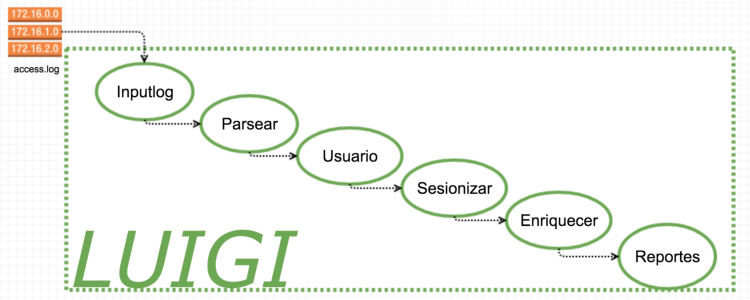
\includegraphics[width=1\textwidth]{Figures/unnamed-chunk-1-1}
\caption{Pipeline del análisis de clickstream}
\end{figure}

\section{Conclusión}

 Con lo investigado dentro de este capítulo, se ha demostrado que el análisis de clickstream es necesario realizarlo con la información generada por el Dspace, ya que como se tiene la completa administración del portal, por medio de los access log, se pueden llevar a cabo un conocimiento profundo de los usuarios con la finalidad de entender sus necesidades de búsqueda y conocer el día a día de sus actividades ya que al tener este tipo de información, se pueden crear recomendaciones para los usuarios recurrentes y los nuevos usuarios. A su vez, también este tipo de análisis ayuda de manera interna (en cuanto a administración), de como está operando el portal ya que es posible detectar posibles problemas por medio de los códigos de respuesta.


\section{Problemas}\label{Problemas que pueden surgir}

Existen 2 tipos principales de archivos logs que son de accesos y error, y dentro de estos se encuentran a su vez otros tipos de archivos; 
por ejemplo, para el caso del tipo access log se encuentran CustomLog (que son los utilizados en el presente estudio), LogFormat y SetEnvIf.
Como la categoría principal es la de access CustomLog, los problemas radican cuando se piensa que se tiene un CustomLog y en realidad es otro tipo de archivo, por lo que al realizar el paso que estructura los datos, el formato es distinto y se tenga un error en cuanto a estructura.

Otro problema está en el paso de detección de usuarios, un mismo usuario puede acceder a un determinado portal desde diferentes computadoras, por ejemplo, desde su casa o la oficina; esto no implica que el análisis de los logs, sean inútiles, pero su funcionamiento está diseñado cuando se identifican a usuarios  registrados o se les realiza alguna recomendación.



\section{Trabajo futuro}\label{trabajo futuro}

Las líneas futuras de investigación existentes que pueden contemplar el análisis, son muchas; sin embargo, se puntualizaran las necesarias a realizar en un futuro cercano:

\begin{itemize}
\item Crear un modelo de recomendaciones a los usuarios basados en filtros colaborativos
\item Tener un seguimiento del éxito de las recomendaciones
\item Identificación de nuevos usuarios para asignar recomendación con base en los usuarios ya existentes.
\item Medición de los códigos de respuesta para conocer posibles errores internos del portal.
\end{itemize}